\chapter{Relações}
\label{cap:relacoes}

Relações entre elementos de conjuntos ocorrem em muitos contextos. Todos dias
lidamos com relações como por exemplo: uma pessoa e o seu número de telemóvel,
um empregado(a) e o seu salário, etc. Em matemática estudamos relações como as
que existem entre um número inteiro positivo e um seu divisor, um inteiro e o
seu quadrado, um valor real $x$ e o valor $f(x)$ onde $f$ é uma função, etc.

As relações são representadas utilizando uma estrutura chamada de
\emph{relação}, que é simplesmente um subconjunto do produto cartesiano de
conjuntos. As relações podem ser utilizadas para resolver problemas tais como:
determinar quais pares de cidades estão ligadas pela mesma companhia área numa
rede, armazenamento de informações em bases de dados, etc.

\section{Relações e suas propriedades}

A forma mais directa de expressar uma relação entre elementos de dois conjuntos
é por utilizar pares ordenados (dois elementos). Por esta razão, os conjuntos de
pares ordenados são chamados de \emph{relações binárias}. Nesta secção
apresentamos a terminologia básica utilizada para descrever as relações binárias.

\label{def41}
\begin{defn}
Sejam $A$ e $B$ conjuntos, uma relação binária de $A$ para $B$ é um subconjunto
de $A \times B$.
\end{defn}

Por outras palavras, uma relação binária de $A$ para $B$ é um conjunto $R$ de
pares ordenados onde o primeiro elemento de cada par ordenado provém de $A$ e o
segundo elemento provém de $B$. Utilizamos a notação $a$ $R$ $b$ para denotar
que $(a,b) \in R$ e $a \centernot{R} b$ para denotar que $(a,b) \notin R$. Além
disso, quando $(a,b)$ pertecem a $R$, dizemos que $a$ \emph{está relacionado} à
$b$ por intermédio de $R$.

As relações binárias representam relacionamentos entre elementos de dois
conjuntos. Apresentaremos mais adiante as relações n-árias que expressam
relacionamentos entre elementos de mais de dois conjuntos. Iremos omitir a
palavra \emph{binária} sempre que não houver perigo de má interpretação. Os
exemplos a seguir ilustram o conceito de \emph{relação}.

\label{exem41}
\begin{exmp}
Sejam $A$ o conjunto dos estudantes da tua escola, e $B$ o conjunto das
disciplinas. Seja $R$ a relação que consiste nos pares $(a,b)$, onde $a$ é um
estudante inscrito na disciplina $b$. Por exemplo, se João e David estão
inscritos na disciplina de Estruturas Discretas (ED), os pares (João, ED) e
(David, ED) pertecem a $R$. Note que se David não está inscrito na disciplina de
ED, então o par (David, ED) não pertence a $R$. Se um estudante não está
inscrito em nenhuma disciplina, não existirá nenhum par em $R$ com este
estudante como primeiro elemento. Da mesma forma se uma disciplina não existe,
não existirá nenhum par em $R$ com esta disciplina como segundo elemento.
\end{exmp}

\label{exem42}
\begin{exmp}
Sejam  $A = \{0,1,2\}$ e $B = \{a,b\},$ então $\{(0,a), (0,b), (1,a), (2,b)\}$ é
uma relação de $A$ para $B$. Isto significa que, por exemplo, $0$ $R$ $a$, mas
$1 \centernot{R} b$.
\end{exmp}

\section{Relações sobre um conjunto}

\label{def42}
\begin{defn}
Uma \emph{relação} num conjunto $A$ é uma relação de $A$ para $A$.
\end{defn}

Por outras palavras, uma relação sobre um conjunto $A$ é um subconjunto de $A
\times A$.

\label{exem43}
\begin{exmp}
Seja $A$ o conjunto $\{1,2,3,4\}$. Que pares ordenados fazem parte da relação $R
= \{(a,b)$ | $a$ divide $b\}$?
	\begin{description}
	\item[Solução:]Como $(a,b)$ pertence a $R$ se e somente se $a$ e $b$ forem
	inteiros positivos não maiores que 4 tal que $a$ divida $b$, vemos que
	\[R=\{(1,1), (1,2), (1,3), (1,4), (2,2), (2,4), (3,3), (4,4)\}.\] Os pares
	nesta relação são apresentados graficamente e em forma tabular na Figura
	\ref{fig41}.
	\end{description}
\end{exmp}

\begin{figure}[H]
	\centering
	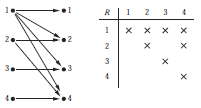
\includegraphics[scale=2.5]{chapter/imagens/41}
	\caption{Apresentando os pares ordenados na relação $R$ no exemplo
	\ref{exem43}.}
	\label{fig41}
\end{figure}

\label{exem44}
\begin{exmp}
Considere as seguintes relações no conjunto dos números inteiros:\\
	$R_1 = \{(a,b)$ | $a \leq b\}$,\\
	$R_2 = \{(a,b)$ | $a > b\}$,\\
	$R_3 = \{(a,b)$ | $a = b $ ou $ a = -b\}$,\\
	$R_4 = \{(a,b)$ | $a = b\}$,\\
	$R_5 = \{(a,b)$ | $a = b + 1\}$,\\
	$R_6 = \{(a,b)$ | $a + b \leq 3\}$,\\
	Qual destas relações contém cada um dos pares $(1,1), (1,2), (2,1), (1,-1)$ e
$(2,2)?$

\begin{description}
\item[Solução:]O par $(1,1)$ está em $R_1, R_3, R_4$ e $R_6$; $(1,2)$ está em
$R_1$ e $R_6$; $(2,1)$ está em $R_2, R_5$ e $R_6$;$(1,-1)$ está em $R_2, R_3$ e
$R_6$; e finalmente, $(2,2)$ está em $R_1, R_3$ e $R_4$.
\end{description}
\end{exmp}


\section{Propriedades das relações}
Existem várias propriedades que são utilizadas para classificar as relações
sobre um conjunto. Iremos apresentar as mais importantes de seguida.

Nalgumas relações um elemento está sempre relacionado consigo próprio. Por
exemplo, seja $R$ a relação no conjunto de todas as pessoas, consistindo nos pares
$(x,y)$ onde $x$ e $y$ são filhos da mesmo pai e da mesma mãe, então $x$ $R$ $y$
para todas as pessoas $x$.

\label{def43}
\begin{defn}
A relação $R$ num conjunto $A$ é chamada de \emph{reflexiva} se $(a,a) \in R$
para todo o elemento $a \in A$.
	
\begin{description}
\item[Nota:]Utilizando quantificadores vemos que uma relação $R$ num conjunto
$A$ é reflexiva se $\forall a((a,a) \in R)$, onde o universo em discurso é o
conjunto de todos os elementos em $A$.
\end{description}
\end{defn}

Vemos que a relação em $A$ é reflexiva se todo elemento de $A$ está relacionado
consigo próprio. Os exemplos a seguir ilustram o conceito de uma relação
reflexiva.

\label{exem45}
\begin{exmp}
Considere as seguintes relações em $\{1,2,3,4\}$:
	\begin{itemize}
		\item $R_1 = \{(1,1),(1,2),(2,1),(2,2),(3,4),(4,1),(4,4)\},$
		\item $R_2 = \{(1,1),(1,2),(2,1)\},$
		\item $R_3 = \{(1,1),(1,2),(1,4),(2,1),(2,2),(3,3),(4,1),(4,4)\},$
		\item $R_4 = \{(2,1),(3,1),(3,2),(4,1),(4,2),(4,3)\},$
		\item $R_5 = \{(1,1),(1,2),(1,3),(1,4),(2,2),(2,3),
		(2,4),(3,3),(3,4),(4,4)\},$
		\item $R_6 = \{(3,4)\}.$
	\end{itemize}
	Quais destas relações são reflexivas?
	
\begin{description}
\item[Solução:]As relações $R_3$ e $R_5$ são reflexivas porque ambas contêm
todos os pares na forma $(a,a)$, nomeadamente, $(1,1), (2,2), (3,3)$ e $(4,4)$.
As outras relações não são reflexivas porque não contêm todos estes pares
ordenados. Em particular $R_1, R_2, R_4$ e $R_6$ não são reflexivas porque
por exemplo $(3,3)$ não faz parte de nenhuma destas relações.
\end{description}
\end{exmp}

\label{exem46}
\begin{exmp}
	Quais das relações no exemplo \ref{exem45} são reflexivas?
	\begin{description}
	\item[Solução:]As relações reflexivas do exemplo \ref{exem45} são $R_1$ (porque
	$a \leq a$ para todo inteiro $a$), $R_3$ e $R_4$. Para cada uma das outras
	relações no exemplo citado é fácil encontrar um par da forma $(a, a)$ que não
	faz parte de nenhuma das relações.
	\end{description}
\end{exmp}

\label{def44}
\begin{defn}
	A relação $R$ num conjunto $A$ é chamada de \emph{simétrica} se $(b,a) \in R$
	sempre que $(a,b) \in R$, para todos $a, b \in A.$ A relação $R$ num conjunto
	$A$ tal que para todo $a,b \in A$, se $(a,b) \in R$ e $(b,a) \in R$, então $a =
	b$, é chamada de \emph{antissimétrica}.
	
	\begin{description}
	\item[\emph{Nota:}]Utilizando quantificadores vemos que uma relação $R$ num
	conjunto $A$ é simétrica se $\forall{a}\forall{b}((a,b) \in R \to (b,a) \in
	R))$. Similarmente, a relação $R$ num conjunto $A$ é antissimétrica se
	$\forall{a}\forall{b}(((a,b) \in R \land (b,a) \in R) \to (a = b)).$
	\end{description}
\end{defn}


Tenha em atenção que uma relação é simétrica se e somente se $a$ está
relacionado à $b$ implica que $b$ está relacionado à $a$. A relação é
antissimétrica se e somente se não existírem pares de distintos elementos $a$ e
$b$ com $a$ relacionado a $b$ e $b$ relacionado a $a$. Isto é, a única forma de
ter $a$ relacionado à $b$ e $b$ relacionado a $a$ é se $a$ e $b$ forem os mesmos
elementos. Os termos \emph{simétrica} e \emph{antissimétrica} não são opostos,
porque a relação pode ter ambas propriedades ou não. A relação só não pode ser
ao mesmo tempo simétrica e antissimétrica se contém algum par da forma $(a,b),$
onde $a \centernot{=} b$.

\label{exem47}
\begin{exmp}
Quais das relações no exemplo \ref{exem45} são simétricas e quais são
antissimétricas?

\begin{description}
\item[Solução:]As relações $R_2$ e $R_3$ são simétricas, porque em
cada caso $(b,a)$ pertence a relação sempre que $(a,b)$ está na relação. Para
$R_2$, a única coisa a verificar é se ambos $(2,1)$ e $(1,2)$ estão na relação.
Para $R_3$, é necessário verificar que $(1,2)$ e $(2,1)$ pertencem a relação, e
$(1,4)$ e $(4,1)$ pertencem a relação. Pode-se facilmente verificar que as
outras relações não são simétricas. Isto pode ser feito por encontrar um par
$(a,b)$ na relação para o qual não exista um par $(b,a)$. $R_4, R_5$ e $R_6$ são
todas antissimétricas. Para cada uma destas relações não existe um par de
elementos $a$ e $b$ com $a \centernot{=} b$ tal que ambos $(a,b)$ e $(b,a)$
pertencem a relação. O leitor pode verificar que nenhuma das outras relações é
antissimétrica. Isto pode ser feito por encontrar um par $(a,b)$ com $a
\centernot{=} b$ tal que $(a,b)$ e $(b,a)$ estão ambos na relação.
\end{description}
\end{exmp}

\label{def45}
\begin{defn}
A relação $R$ num conjunto $A$ é chamada de \emph{transitiva} se sempre que
$(a,b) \in R$ e $(b,c) \in R$, então $(a,c) \in R$, para todos $a, b, c \in
A$.

\begin{description}
\item[\emph{Nota:}]Utilizando quantificadores vemos que uma relação $R$ num
conjunto $A$ é transitiva se temos $\forall{a}\forall{b}\forall{c}(((a,b) \in R
\land (b,c) \in R) \to (a,c) \in R)$.
\end{description}
\end{defn}

\label{exem48}
\begin{exmp}
Quais das relações no exemplo \ref{exem45} são transitivas?

\begin{description}
\item[Solução:]As relações $R_4, R_5$ e $R_6$ são transitivas. Para cada uma
destas relações, poderemos provar que são transitivas por verificar que se
$(a,b)$ e $(b,c)$ pertencem a esta relação, então $(a,c)$ também fazem parte.
Por exemplo, $R_4$ é transitiva, porque $(3,2)$ e $(2,1)$, $(4,2)$ e $(2,1)$,
$(4,3)$ e $(3,1)$, e $(4,3)$ e $(3,2)$ fazem parte da relação tal como os pares
$(3,1),(4,1)$ e $(4,2)$. Como exercício, verifique se $R_5$ e $R_6$ são
transitivas. $R_1$ não é transitiva porque $(3,4)$ e $(4,1)$ pertencem a $R_1$,
mas $(3,1)$ não. $R_2$ não é transitiva porque $(2,1)$ e $(1,2)$ pertencem a
$R_2$, mas $(2,2)$ não fazem parte. $R_3$ não é transitiva porque $(4,1)$ e
$(1,2)$ pertencem a $R_3$, mas $(4,2)$ não.
\end{description}
\end{exmp}


	
\section{Combinação de relações}

Como as relações de $A$ para $B$ são subconjuntos de $A \times B$, duas
relações de $A$ para $B$ podem ser combinadas da mesma forma como os conjuntos
podem ser combinados. Considere os exemplos abaixo:

\label{exem49}
\begin{exmp}
Sejam $A = \{1,2,3\}$ e $B = \{1,2,3,4\}$. As relações $R_1 = \{(1, 1), (2, 2),
(3, 3)\}$ e $R_2 = \{(1, 1), (1, 2), (1, 3), (1, 4)\}$ podem ser combinadas
para obter:
\begin{itemize}
	\item $R_1 \cup R_2 = \{(1, 1), (1, 2), (1, 3), (1, 4), (2, 2), (3, 3)\}$
	\item $R_1 \cap R_2 = \{(1,1)\}$
\end{itemize}
\end{exmp}

\label{exem410}
\begin{exmp}
Seja $R_1$ a relação ``menor que'' no conjunto dos números reais e seja $R_2$ a
relação ``maior que'' no conjunto dos números reais, isto é, $R_1 = \{(x,y)
\mid x < y\}$ e $R_2 = \{(x,y) \mid x > y\}$. O que são $R_1 \cup R_2$, $R_1
\cap R_2$, $R_1 - R_2$ e $R_2 - R_1$?

\begin{description}
\item[\emph{Solução:}]Notamos que $(x,y) \in R_1 \cup R_2$ se e somente se
$(x,y) \in R_1$ ou $(x,y) \in R_2$. Assim, $(x,y) \in R_1 \cup R_2$ se e somente
se $x < y$ ou $x > y$. Como a condição $x < y$ ou $x > y$ é o mesmo que a
condição $x \neq y$, segue-se que $R_1 \cup R_2 = \{(x,y) \mid x \neq y\}$. Por
outras palabras, a união da relação ``menor que'' com a relação ``maior que'' é
a relação ``diferente de''.
De seguida, note que é impossível para um par $(x,y)$ pertencer a ambos os pares
$R_1$ e $R_2$ porque é impossível que $x<y$ e $x>y$. Segue-se que $R_1 \cap R_2
= \emptyset$. Também notamos que $R_1 - R_2 = R_1$ e $R_2 - R_1 = R_2$.
\end{description}
\end{exmp}

Existe uma outra forma de combinar relações que é análoga a composição de
funções.

\label{def46}
\begin{defn}
Seja $R$ a relação de um conjunto $A$ para um conjunto $B$ e $S$ uma relação de
$B$ para $C$. A \emph{composta} de $R$ e $S$ é a relação que consiste nos pares
ordenados $(a,c)$, onde $a \in A$, $c \in C$ e para os quais existe um elemento
$b \in B$ tal que $(a,b) \in R$ e $(b,c) \in S$. Denotamos a composta de $R$ e
$S$ por $S \circ R$.
\end{defn}

Calcular a composta de duas relações requer que encontremos elementos que são o
segundo elemento de um par ordenado na primeira relação e o primeiro elemento de
pares ordenados na segunda relação, como os exemplos a seguir ilustram.

\label{exem411}
\begin{exmp}
Qual é a composta das relaçãoes $R$ e $S$, onde $R$ é a relação de $\{1,2,3\}$
para $\{1,2,3,4\}$ com $R = \{(1,1),(1,4),(2,3),(3,1),(3,4)\}$ e $S$ é uma
relação de $\{1,2,3,4\}$ para $\{0,1,2\}$ com $S =
\{(1,0),(2,0),(3,1),(3,2),(4,1)\}$?

\begin{description}
\item[\emph{Solução:}] $S \circ R$ é construída utilizando todos os pares
ordenados em $R$ e pares ordenados em $S$, onde o segundo elemento do par
ordenado em $R$ é o mesmo que o primeiro elemento do par ordenado em $S$. Por
exemplo, os pares ordenados $(2,3)$ em $R$ e $(3,1)$ em $S$ produzem o par
ordenado $(2,1)$ em $S \circ R$. Computando todos os pares ordenados na composta
de $S$ e $R$ obtemos,
\begin{center}
$S \circ R = \{(1,0), (1,1), (2,1), (2,2), (3,0), (3,1)\}$.
\end{center}
\end{description}
\end{exmp}


\label{exem412}
\begin{exmp}
\textbf{Compondo uma relação consigo própria} Seja $R$ a relação no conjunto de
todas as pessoas tal que $(a,b) \in R$ se a pessoa $a$ é o pai da pessoa $b$.
\end{exmp}



\section{Representação de relações}

\subsection{Introdução}

\textbf{Nota}: Nesta secção, utilizaremos sómente as relações binárias. Por
esta razão a palavra relação irá apenas referir-se a relações binárias.

Existem muitas formas de representar uma relação entre conjuntos finitos. Uma
forma é por listar os pares ordenados.
Outra forma de representar uma relação é por meio de tabelas como vimos na
secção anterior. Nesta secção vamos apresentar dois métodos de representação
alternativos: matrizes zero-um e gráfos direccionados. No geral, as matrizes
são apropriadas para a representação de relações em programas de computador.
Por outro lado, algumas pessoas acham a representação de relações utilizando
grafos direccionados mais útil ao entendimento das propriedades dessas relações.

\subsection{Representação de relações por meio de matrizes}

A relação entre conjuntos finitos pode ser representada utilizando matrizes
zero-um. Suponha que $R$ é uma relação de $A = \{a_1, a_2, \ldots, a_m\}$ para
$B = \{b_1, b_2, \ldots, b_n\}$. (Aqui os elementos dos conjuntos A e B são
listados duma forma particular, embora arbitrária. Além dos mais, quando $A =
B$ utilizamos a mesma ordenação para $A$ e $B$.) A relação $R$ pode ser
representada pela matriz $M_R = [m_{ij}]$,\\


$m_{ij} = \begin{cases}
	1$ se $(a_i, b_j) & \in R,\\
	0$ se $(a_i, b_j) & \notin R.
\end{cases}$


Por outras palavras, a matriz zero-um que representa $R$ tem o valor 1 em
$(i,j)$ quando $a_i$ está relacionado a $b_j$, e o valor 0 nesta posição se
$a_i$ não está relacionado a $b_j$. Esta representação depende da ordem
utilizada para $A$ e $B$. A utilização de matrizes para representar relações é
ilustrada no exemplos a seguir.

\begin{description}
	\elabel{exe610}
	\item[Exemplo \ref{exe610}] {Suponha que $A = \{1,2,3\}$ e $B = \{1,2\}$. Seja
	R a relação de $A$ para $B$ contendo os pares $(a,b)$ se $a \in A$, $b \in B$
	e $a > b$. Qual é a matriz que representa $R$ se $a_1 = 1$, $a_2 = 2$, $a_3 =
	3$ e $b_1 = 1$ e $b_2 = 2?$}
\end{description}

\emph{Solução:} Como $R = \{(2, 1), (3, 1), (3, 2)\}$, a matriz para $R$ é:

\[
M_R = \begin{bmatrix}
	0 & 0\\
	1 & 0\\
	1 & 1
\end{bmatrix}
\]

Os 1s em $M_R$ mostram que os pares $(2,1), (3,1)$ e $(3,2)$ pertencem a $R$. Os 0s mostram que os outros pares não
pertencem a $R$.

\begin{description}
	\elabel{exe611}
	\item[Exemplo \ref{exe611}]{Sejam $A = \{a_1, a_2, a_3\}$ e $B = \{b_1, b_2,
	b_3, b_4, b_5\}$, quais pares ordenados estão na relação $R$ representada pela
	matriz}
\end{description}

\[
	M_R = \begin{bmatrix}
	0 & 1 & 0 & 0 & 0\\
	1 & 0 & 1 & 1 & 0\\
	1 & 0 & 1 & 0 & 1
	\end{bmatrix}?
\]
	
\emph{Solução} Como $R$ consiste nos pares ordenados $(a_i, b_j)$ com $m_{ij} =
1$ daí resulta que $R = \{(a_1,b_2), (a_2,b_1), (a_2, b_3), (a_2, b_4), (a_3,
b_1), (a_3, b_3), (a_3, b_5)\}$

A matriz de uma relação em um conjunto, que é uma matriz quadrada, pode ser
utilizada para determinar se a relação possui certas propriedades. Sabemos que
uma relação $R$ num conjunto $A$ é reflexiva se $(a,a) \in R$ sempre que $a \in
A$, então, $R$ é reflexiva se e somente se $(a_i, a_i) \in R$ para $i =
1,2,\ldots,n$. Assim, $R$ é reflexiva se e somente se $m_{ii} = 1$, para $i =
1,2,\ldots,n$. Por outras palavras, $R$ é reflexiva se todos os elementos da
diagonal principal de $M_R$ são iguais a $1$, como ilustrado na Figura
\ref{Figura61}. Note que os elementos fora da diagonal podem ser $0s$ ou $1s$.

\begin{figure}[H]
	\centering
	\[
	\begin{bmatrix}
	 1	& 	& 	&	&	&	&	&\\
	 	& 1 &	&	&	&	&	&\\
		&	& 1 &	&	&	&	&\\
		&	&  	& .	&	&	&	&\\
		&	&	& 	& . &	&	&\\
		&	&	&	&	& . &	&\\
		&	&	& 	&	&	& 1	&\\
		&	&	&	&	&	&	& 1 
	\end{bmatrix}
	\]
	\caption{A matriz zero-um para uma relação reflexiva. (Os elementos fora da diagonal podem ser 0 ou 1.)}
	\label{Figura61}
\end{figure}

A relação $R$ é simétrica se $(a,b) \in R$ implica que $(b, a) \in R$.
Consequentemente, a relação $R$ no conjunto $A = \{a_1, a_2, \ldots, a_n\}$ é
simétrica se e somente se $(a_j, a_i) \in R$ sempre que $(a_i, a_j) \in R$. Em
termos dos valores de $M_R$, $R$ é simétrica se e somente se $m_{ji} = 1$
sempre que $m_{ij} = 1$. Isto também significa que $m_{ji} = 0$ sempre que
$m_{ij} = 0$. Consequentemente, $R$ é simétrica se e somente se $m_{ij} =
m_{ji}$, para todos os pares de inteiros $i$ e $j$ com $i = 1,2,\ldots,n$ e
$j=1,2,\ldots,n$. $R$ é simétrica se e somente se $M_R = (M_R)^t$ onde
$(M_R)^t$ é matriz transposta de $M_R$.

A relação $R$ é antissimétrica se e somente se $(a, b) \in R$ e $(b, a) \in R$
implica que $a = b$. Consequentemente, a matrix de uma relação antissimétrica
tem a propriedade de que se $m_{ij} = 1$ com $i \ne j$, então $m_{ji} = 0$.
Ou, em outras palavras, $m_{ij} =0$ ou $m_{ji} =0$ quando $i \ne j$. A forma da
matriz para uma relação antissimétrica é ilustrada na Figura \ref{Figura62}.

\begin{figure}[H]
	\centering
	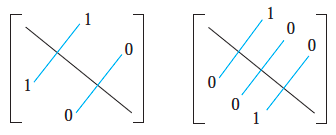
\includegraphics[scale=0.6]{chapter/imagens/62}
	\caption{A matriz zero-um para uma relação simétrica e antissimétrica.}
	\label{Figura62}
\end{figure}

\begin{description}
	\elabel{exe612}
	\item[Exemplo \ref{exe612}]{Suponha que a relação $R$ é representada pela
	matriz}
\end{description}
\[
	M_R = \begin{bmatrix}
	1 & 1 & 0\\
	1 & 1 & 1\\
	0 & 1 & 1
	\end{bmatrix}?
\]

$R$ é reflexiva, simétrica e/ou antisimétrica?

\emph{Solução:} Como todos os elementos das diagonais nesta matriz são iguais a
$1$, $R$ é reflexiva.
Além do mais, como $M_R$ é simétrica, então $R$ é simétrica. É também fácil
notar que $R$ não é antissimétrica.

As operações booleanas estudadas anteriormente também podem ser utilizadas para
encontrar as matrizes que representam a união e a intersecção de duas relações.
Suponha que $R_1$ e $R_2$ são relações num conjunto $A$ representada pelas
matrizes $M_{R_1}$ e $M_{R_2}$, respectivamente. A matriz que representa a
união destas duas relações possui o valor $1$ nas posições em que  $M_{R_1}$ ou
$M_{R_2}$ possuem o valor $1$. A matriz que representa a intersecção destas
duas relações possui o valor $1$ nas posições em que  $M_{R_1}$ e $M_{R_2}$
possuem o valor $1$.
Sendo assim, as matrizes que representam a união e a intersecção destas duas
relações são:

\begin{itemize}
  \item $M_{R_1 \cup R_2} = M_{R_1} \lor M_{R_2}$ e,
  \item $M_{R_1 \cap R_2} = M_{R_1} \land M_{R_2}$
\end{itemize}


\subsection{Representação de relações por meio de grafos direccionados}

Vimos anteriormente que uma relação pode ser representada por uma listagem de
todos os seus pares ordenados ou por meio de uma matriz zero-um. Existe outra
forma importante de representar uma relação utilizando uma representação
pictural. Cada elemento do conjunto é representado por um ponto, e cada par
ordenado é representado utilizando um arco cuja direcção é indicada por uma
seta.
Utilizamos essa representação sempre que pensamos em relações como grafos
direccionados ou dígrafos, num conjunto finito.


\begin{description}
	\dlabel{def66}
	\item[Definição \ref{def66}]{Um \emph{grafo direccionado}, ou \emph{dígrafo},
	consiste num conjunto $V$ de \emph{vértices} (ou \emph{nós}) e um conjunto $E$
	de pares ordenados dos elementos de $V$ chamados de \emph{arestas} (ou
	\emph{arcos}). O vértice $a$ é chamado de \emph{vértice inicial} da aresta
	$(a,b)$, e o vértice $b$ é chamado de \emph{vértice terminal} desta aresta.}
\end{description}

Uma aresta da forma $(a, a)$ é representada utilizando um arco do vértice $a$ de volta à sí mesmo. Tal aresta é chamada de 
\textbf{laço} ou \textbf{loop}.


\begin{description}
	\elabel{exe613}
	\item[Exemplo \ref{exe613}]{O grafo direccionado com os vértices $a, b, c$ e
	$d$ e as arestas \\$(a,b), (a,d), (b,b), (b,d), (c,a), (c,b)$ e $(d,b)$ é
	apresentado na Figura \ref{Figura63}}
\end{description}

\begin{figure}[H]
	\centering
	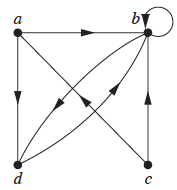
\includegraphics[scale=0.6]{chapter/imagens/63}
	\caption{Um grafo direccionado.}
	\label{Figura63}
\end{figure}


A relação $R$ no conjunto $A$ é representada pelo grafo ordenado que possui
elementos de $A$ como seus vértices e os pares ordenados $(a,b)$, onde $(a,b)
\in R$, como arestas. Esta atribuição configura uma correspondência
\emph{um-para-um} entre as relações no conjunto $A$ e os grafos direcionados que
possuem $A$ como o seu conjunto de vértices. Assim, cada afirmação sobre relações corresponde a
uma afirmação sobre grafos direccionados, e vice-versa. Grafos direccionados
fornecem uma exibição visual das relações e por isso são utilizados no estudo
das relações e de suas propriedades. A utilização de grafos direccionados na
represetntação de relações num conjunto é ilustrada nos seguintes exemplos.

\begin{description}
	\elabel{exe614}
	\item[Exemplo \ref{exe614}]{
	O grafo direccionado da relação\\
	$R = {(1, 1), (1, 3), (2, 1), (2, 3), (2, 4), (3, 1), (3, 2), (4, 1)}$\\
	no conjunto $\{1, 2, 3, 4\}$ é ilustrado na Figura \ref{Figura64}
	}
\end{description}

\begin{figure}[H]
	\centering
	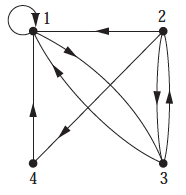
\includegraphics[scale=0.6]{chapter/imagens/64}
	\caption{Um grafo direccionado.}
	\label{Figura64}
\end{figure}

\begin{description}
	\elabel{exe615}
	\item[Exemplo \ref{exe615}]{
	Quais são os pares ordenados na relação $R$ representada pelo grafo direccionado da Figura \ref{Figura65}}
\end{description}

\begin{figure}[H]
	\centering
	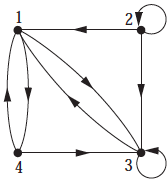
\includegraphics[scale=0.6]{chapter/imagens/65}
	\caption{Um grafo direccionado da relação R.}
	\label{Figura65}
\end{figure}

\emph{Solução:} Os pares ordenados $(x,y)$ na relação são \[$R = {(1,
3), (1, 4), (2, 1), (2, 2), (2, 3), (3, 1), (3, 3), (4, 1), (4, 3)}\]

Cada um destes pares corresponde à uma aresta do grafo direccionado sendo
$(2,2)$ e $(3,3)$ dois laços.

O grafo direccionado que representa uma relação pode ser utilizado para
determinar se a relação possui certas propriedades.
Por exemplo, a relação é reflexiva se e somente se existe um laço em cada
vértice do grafo direccionado, de tal forma que todos os pares ordenados da
forma $(x,x)$ ocorrem na relação. A relação é simétrica se e somente se para
cada aresta entre vértices distintos no digrafo existe uma aresta na direcção
oposta, tal que $(y,x)$ existe na relação sempre que $(x,y)$ existe na relação.
Da mesma forma, uma relação é antissimétrica se e somente se não existem duas
arestas em direcções opostas entre vértices distintos. Finalmente, uma relação
é transitiva se e somente se sempreque que existe uma aresta de um vértice $x$
para um vértice $y$ e uma aresta de um vértice $y$ para um vértice $z$, existe
uma aresta de $x$ para $z$ (completando um triângulo onde cada lado é uma aresta
na direcção correcta).


\begin{description}
	\elabel{exe616}
	\item[Exemplo \ref{exe616}]{Determine se os grafos direccionados apresentados
	nas Figuras \ref{Figura66} e \ref{Figura67} são reflexivos, simétricos,
	antissimétricos e/ou transitivos}.
\end{description}

\begin{figure}[H]
	\centering
	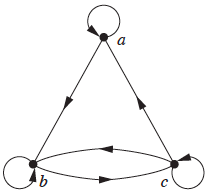
\includegraphics[scale=0.6]{chapter/imagens/66}
	\caption{Um grafo direccionado da relação R.}
	\label{Figura66}
\end{figure}

\begin{figure}[H]
	\centering
	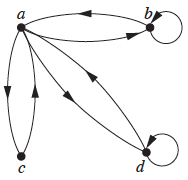
\includegraphics[scale=0.6]{chapter/imagens/67}
	\caption{Um grafo direccionado da relação S.}
	\label{Figura67}
\end{figure}

\emph{Solução:} Como existem laços em todos os vértices do grafo direccionado
de $R$, ele é reflexivo. $R$ não é simétrico nem anti-simétrico porque existe
uma aresta de $a$ para $b$ mas não de $b$ para $a$, mas existem arestas em
ambas direcções que conectam $b$ e $c$. Finalmente, $R$ não é transitivo porque
existe uma aresta de $a$ para $b$ e uma aresta de $b$ para $c$, mas não existe
uma aresta de $a$ para $c$. Como não existem laços em todos os vértices do grafo
direccionado de S, esta relação não é reflexiva. É simétrica mas não
antissimétrica, porque cada aresta entre vértices distintos é acompanhada por
uma aresta na direcção oposta. Não é díficil notar também que o grafo
direccionado de $S$ não é transitivo, porque $(c,a)$ e $(a,b)$ pertencem a $S$,
mas $(c,b)$ não pertence a $S$.

Estudaremos os grafos em mais detalhes no capítulo \ref{cap:grafos}.


\section{Fecho de relações}

\subsection{Introdução}

Uma rede de computadores de uma empresa possui centros de dados em Benguela,
Bengo, Cabinda, Cunene, Huíla e Luanda.
Existem ligações directas de Benguela para o Bengo, de Benguela para o Bengo,
de Benguela para Cunene, do Bengo para o Cunene, de Cunene para Cabinda e da
Huíla para Luanda. Seja $R$ a relação que contém $(a,b)$ se existe uma ligação
do centro de dados em $a$ com o centro de dados em $b$, como podemos determinar
se existe uma ligação (possívelmente indirecta) composta de uma ou mais linhas
de um centro para outro? Como nem todas as ligações são directas, tal como a
ligação de Benguela para Cabinda que passa por Cunene, $R$ não pode ser
utilizada directamente para responder esta questão.
Na linguagem das relações, $R$ não é transitiva, portanto não contém todos os
pares que podem ser ligado. Tal como iremos mostrar nesta secção, é possível
achar todos os pares de centros de dados que possuem um link por construír uma
relação transitiva $S$ que contém $R$ tal que $S$ é um subconjunto de todas as
relações transitivas que contêm $R$.


\section{Relações de equivalência}

\section{Ordens parciais}